\documentclass[11pt]{scrartcl}

\usepackage[utf8]{inputenc} 
\usepackage[T1]{fontenc}     
\usepackage[french]{babel} 
\usepackage{lmodern}
\usepackage{microtype}
\usepackage{xcolor}
\usepackage{sectsty}
\usepackage{geometry} 
\usepackage{fancyhdr}  
\usepackage{graphicx}        
\usepackage{amsmath, amssymb} 
\usepackage[hidelinks]{hyperref} 

\hypersetup{pdfnewwindow=true}
\setcounter{secnumdepth}{0}   
\definecolor{mainblue}{RGB}{0, 102, 204}
\sectionfont{\color{blue!60!black}\sffamily\Large\bfseries}  
\geometry{margin=2cm}


%%%%%%%%%%%%%%%%%%%%%%%%%%%%%%%%%%%%%%%%%%%%%%%%%%%%%%%%%%%%%%%%%%%%%%%%%%%%%%%%%%%%%%%
%%%%%%%%%%                       EN-TÊTE ET PIED DE PAGE                     %%%%%%%%%%
%%%%%%%%%%%%%%%%%%%%%%%%%%%%%%%%%%%%%%%%%%%%%%%%%%%%%%%%%%%%%%%%%%%%%%%%%%%%%%%%%%%%%%%

\pagestyle{fancy}
\fancyhf{} 

%%% En-tête de page
\fancyhead[L]{\footnotesize IUT de Lannion - Département Informatique}
\fancyhead[R]{\footnotesize 2025} 

%%% Pied de page
\fancyfoot[L]{\footnotesize © Stanislas ROLLAND - Pierre LECHAT - Tous droits réservés} 
\fancyfoot[R]{\footnotesize \thepage}

\renewcommand{\footrulewidth}{0.4pt}


%%%%%%%%%%%%%%%%%%%%%%%%%%%%%%%%%%%%%%%%%%%%%%%%%%%%%%%%%%%%%%%%%%%%%%%%%%%%%%%%%%%%%%%
%%%%%%%%%%                        PAGE DE PRÉSENTATION                       %%%%%%%%%%
%%%%%%%%%%%%%%%%%%%%%%%%%%%%%%%%%%%%%%%%%%%%%%%%%%%%%%%%%%%%%%%%%%%%%%%%%%%%%%%%%%%%%%%

\title{RAPPORT D'ANALYSE DE DONNÉES}
\author{Stanislas ROLLAND - Pierre LECHAT}
\date{Septembre 2025}

\begin{document}

    \maketitle
    \tableofcontents  
    \newpage
 

    %%%%%%%%%%%%%%%%%%%%%%%%%%%%%%%%%%%%%%%%%%%%%%%%%%%%%%%%%%%%%%%%%%%%%%%%%%%%%%%%%%%
    %%%%%%%%%%                          INTRODUCTION                         %%%%%%%%%%
    %%%%%%%%%%%%%%%%%%%%%%%%%%%%%%%%%%%%%%%%%%%%%%%%%%%%%%%%%%%%%%%%%%%%%%%%%%%%%%%%%%%

    \section{Introduction}

        Dans le cadre de notre formation en BUT Informatique à l'IUT de Lannion, nous avons été amenés à réaliser un projet d'analyse de données.\\\\
        Nous avons choisi d'analyser un jeu de données concernant les statistiques des joueurs de football évoluant dans les cinq meilleures ligues européennes durant la saison 2024 - 2025. Ce choix a été motivé par notre intérêt commun pour le football et par la richesse des données disponibles dans ce domaine.\\\\
        Le présent rapport détaille les différentes étapes de notre analyse, depuis la présentation du jeu de données jusqu'aux techniques d'analyse utilisées, en passant par les résultats obtenus et leur interprétation.


    %%%%%%%%%%%%%%%%%%%%%%%%%%%%%%%%%%%%%%%%%%%%%%%%%%%%%%%%%%%%%%%%%%%%%%%%%%%%%%%%%%%
    %%%%%%%%%%                         JEU DE DONNÉES                        %%%%%%%%%%
    %%%%%%%%%%%%%%%%%%%%%%%%%%%%%%%%%%%%%%%%%%%%%%%%%%%%%%%%%%%%%%%%%%%%%%%%%%%%%%%%%%%

    \section{Présentation du jeu de données}

        \subsection{Description du jeu de données}
            Le jeu de données que nous avons choisi d'analyser est un ensemble de données concernant les statistiques des joueurs de football sur la saison 2024 - 2025 les cinq meilleures ligues européennes (Premier League, La Liga, Serie A, Ligue 1, Bundesliga).\\\\
            Notre jeu de données comporte 197 entrées (une par joueur) et les 15 variables suivantes :

            \textbf{\\\underline{Variables qualitatives :}\\}
                \begin{itemize}
                    \item \textbf{Player} : Nom et prénom du joueur.
                    \item \textbf{Nation} : Nationalité du joueur.
                    \item \textbf{Pos} : Position principale du joueur sur le terrain (ex : Attaquant, Défenseur, Gardien).
                    \item \textbf{Squad} : Équipe actuelle du joueur.
                    \item \textbf{Comp} : Compétition dans laquelle le joueur évolue (ex : Premier League, La Liga etc).
                \end{itemize}
            
            \textbf{\\\underline{Variables quantitatives :}\\}
                \begin{itemize}
                    \item \textbf{Id} : Identifiant unique du joueur.
                    \item \textbf{Age} : Âge du joueur.
                    \item \textbf{Born} : Année de naissance du joueur.
                    \item \textbf{MP} : Nombre de matchs joués par le joueur.
                    \item \textbf{Starts} : Nombre de matchs commencés comme titulaire.
                    \item \textbf{Min} : Nombre total de minutes jouées.
                    \item \textbf{90s} : Nombre de périodes de 90 minutes jouées (équivalent à des matchs complets).
                    \item \textbf{Gls} : Nombre total de buts marqués.
                    \item \textbf{Ast} : Nombre total de passes décisives.
                    \item \textbf{G+A} : Somme des buts et des passes décisives.
                \end{itemize}

        \subsection{Exemple d'une entrée du jeu de données}

            \begin{center}
                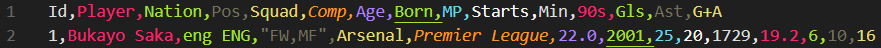
\includegraphics[width=1\textwidth]{images/exemple_entree.png}
                \captionof{figure}{}
            \end{center}    


    %%%%%%%%%%%%%%%%%%%%%%%%%%%%%%%%%%%%%%%%%%%%%%%%%%%%%%%%%%%%%%%%%%%%%%%%%%%%%%%%%%%
    %%%%%%%%%%               TECHNIQUES D'ANALYSE DE DONNÉES                 %%%%%%%%%%
    %%%%%%%%%%%%%%%%%%%%%%%%%%%%%%%%%%%%%%%%%%%%%%%%%%%%%%%%%%%%%%%%%%%%%%%%%%%%%%%%%%%

    \section{Présentation des techniques d'analyse de données}


    %%%%%%%%%%%%%%%%%%%%%%%%%%%%%%%%%%%%%%%%%%%%%%%%%%%%%%%%%%%%%%%%%%%%%%%%%%%%%%%%%%%
    %%%%%%%%%%                  ANALYSE QUANTITATIVE : APC                   %%%%%%%%%%
    %%%%%%%%%%%%%%%%%%%%%%%%%%%%%%%%%%%%%%%%%%%%%%%%%%%%%%%%%%%%%%%%%%%%%%%%%%%%%%%%%%%

    \section{Analyse quantitative des données : l'ACP}

        \subsection{Définition}
            L'Analyse en Composantes Principales (ACP) est une technique statistique utilisée pour réduire la dimensionnalité d'un jeu de données tout en conservant le maximum d'information possible. Elle permet de transformer un ensemble de variables corrélées en un ensemble de variables non corrélées appelées composantes principales.\\\\
            L'ACP est particulièrement utile lorsque l'on travaille avec des données multivariées, c'est-à-dire des données comportant plusieurs variables quantitatives. En réduisant le nombre de dimensions, l'ACP facilite la visualisation et l'interprétation des données, tout en aidant à identifier les structures sous-jacentes et les relations entre les variables.\\


        %%%%%%%%%%%%%%%%%%%%%%%%%%%%%%%%%%%%%%%%%%%%%%%%%%%%%%%%%%%%%%%%%%%%%%%%%%%%%%%%%%%
        %%%%%%%%%%                     CERCLE DE CORRÉLATION                     %%%%%%%%%%
        %%%%%%%%%%%%%%%%%%%%%%%%%%%%%%%%%%%%%%%%%%%%%%%%%%%%%%%%%%%%%%%%%%%%%%%%%%%%%%%%%%%

        \subsection{Cercle de corrélation}
            \subsubsection{Définition}
                Le cercle de corrélation est un outil graphique utilisé dans le cadre de l'ACP pour visualiser les relations entre les variables originales et les composantes principales. Chaque variable est représentée par un vecteur dans un plan défini par les deux premières composantes principales.\\\\
                La position et la longueur des vecteurs permettent d'interpréter la contribution de chaque variable aux composantes principales. Par exemple, des vecteurs proches les uns des autres indiquent des variables fortement corrélées, tandis que des vecteurs perpendiculaires suggèrent une absence de corrélation. La distance d'un vecteur à l'origine reflète l'importance de la variable dans la formation des composantes principales.
                
                \begin{center}
                    \includegraphics[width=0.75\textwidth]{images/cercle_de_corrélation.png}
                    \captionof{figure}{}
                \end{center}

            \subsubsection{Interprétation}
                Dans la figure ci-dessus, on peut observer que les variables "Gls" et "G+A" sont plus ou moins corréléeses car "G+A" est la somme de "Gls" et "Ast". En revanche la variable "Ast" n'est pas corrélées avec ces dernières, ce qui peut être expliqué par le fait que les joueurs qui inscrivent beaucoup de buts inscrivent généralement beaucoup moins de passes décisives.\\\\
                Quant à elle, les variables "MP", "Starts", "Min" et "90s" sont également fortement corrélées entre elles, ce qui reflète le fait que ces variables mesurent différentes facettes du temps de jeu des joueurs.\\\\
                La variable "Age", elle, semble être très faiblement corrélée avec les autres variables, ce qui peut indiquer que l'âge des joueurs n'a pas une influence directe sur leurs performances statistiques dans ce jeu de données.\\
    

        %%%%%%%%%%%%%%%%%%%%%%%%%%%%%%%%%%%%%%%%%%%%%%%%%%%%%%%%%%%%%%%%%%%%%%%%%%%%%%%%%%%
        %%%%%%%%%%                   GRAPHIQUE DES INDIVIDUS                     %%%%%%%%%%
        %%%%%%%%%%%%%%%%%%%%%%%%%%%%%%%%%%%%%%%%%%%%%%%%%%%%%%%%%%%%%%%%%%%%%%%%%%%%%%%%%%%

        \subsection{Graphique des individus}
            \subsubsection{Définition}
                Le graphique des individus est un outil visuel utilisé dans le cadre de l'ACP pour représenter les observations (individus) dans l'espace défini par les composantes principales. Chaque point sur le graphique correspond à une observation du jeu de données, et la position de chaque point est déterminée par ses coordonnées sur les axes des composantes principales.\\\\
                Ce graphique permet d'identifier des groupes d'individus similaires, des tendances générales, ainsi que des observations atypiques ou des outliers. En analysant la distribution des points, on peut tirer des conclusions sur la structure sous-jacente des données et sur les relations entre les différentes observations. 

                \begin{center}
                    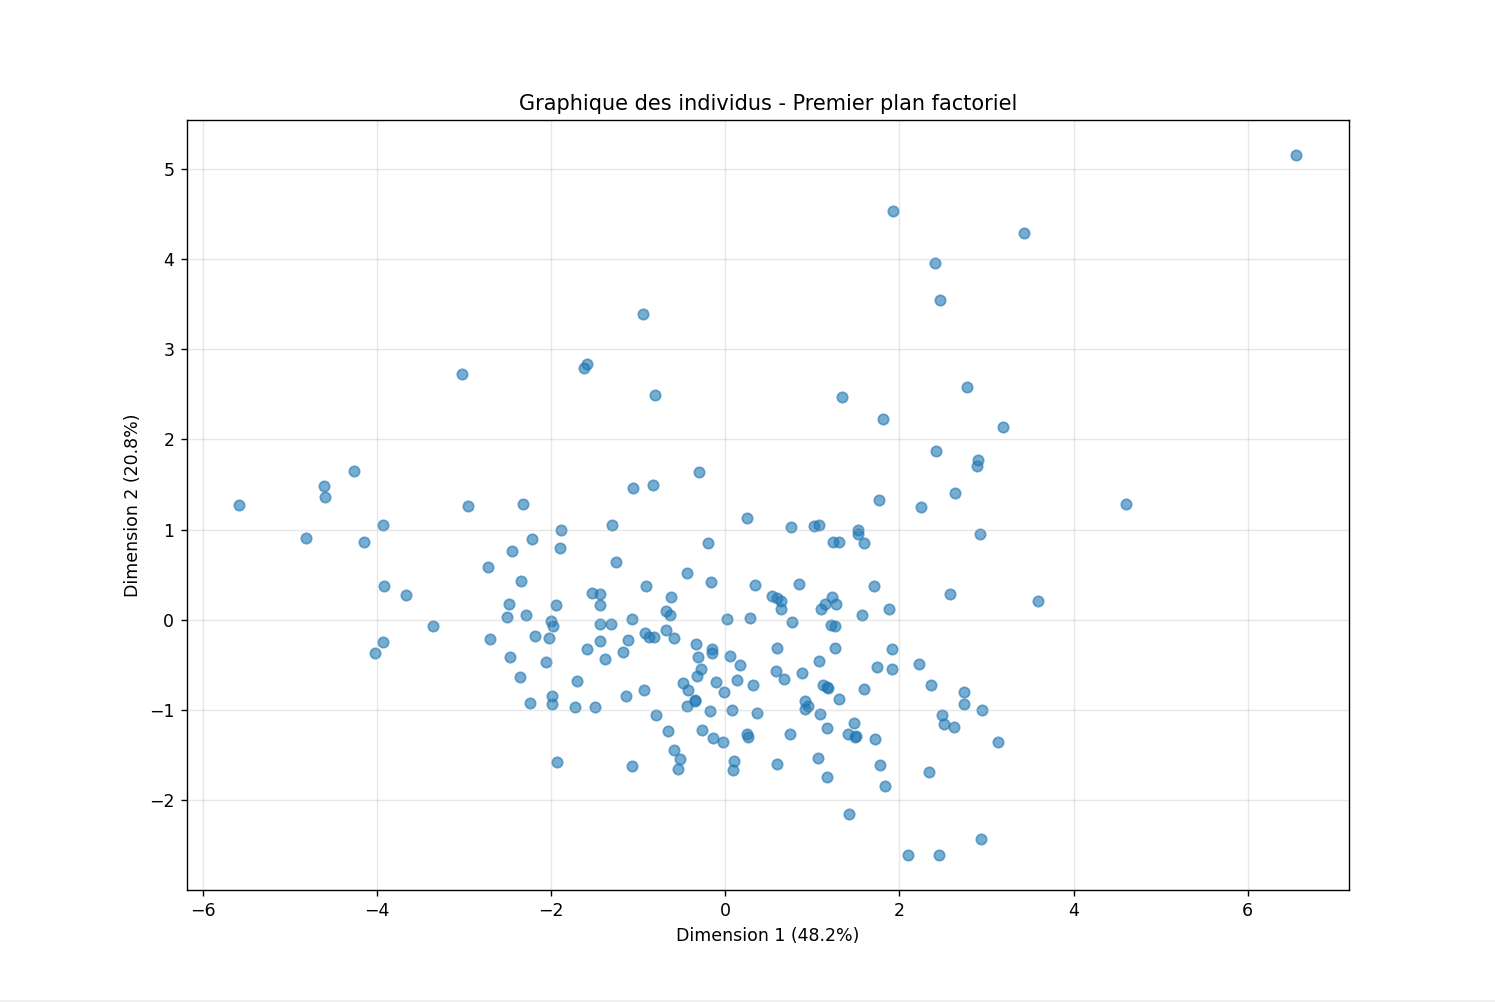
\includegraphics[width=0.75\textwidth]{images/graphiques_des_individus.png}
                    \captionof{figure}{}
                \end{center}

            \subsubsection{Interprétation}
                Dans la figure ci-dessus, on peut observer que les joueurs sont répartis en plusieurs groupes distincts. Par exemple, on peut identifier un groupe de joueurs situés dans la partie supérieure droite du graphique, qui sont probablement des attaquants ou des milieux offensifs, car ils ont des valeurs élevées pour les variables "Gls" et "G+A".\\\\
                En revanche, les joueurs situés dans la partie inférieure gauche du graphique ont des valeurs plus faibles pour ces variables, ce qui suggère qu'ils sont probablement des défenseurs ou des gardiens de but.\\\\
                De plus, on peut remarquer que certains joueurs sont situés loin du centre du graphique, ce qui indique qu'ils ont des performances statistiques atypiques par rapport à la majorité des joueurs. Ces observations peuvent être considérées comme des outliers et méritent une attention particulière pour comprendre les raisons de leurs performances exceptionnelles ou médiocres.\\


        %%%%%%%%%%%%%%%%%%%%%%%%%%%%%%%%%%%%%%%%%%%%%%%%%%%%%%%%%%%%%%%%%%%%%%%%%%%%%%%%%%%
        %%%%%%%%%%                        VALEURS PROPRES                        %%%%%%%%%%
        %%%%%%%%%%%%%%%%%%%%%%%%%%%%%%%%%%%%%%%%%%%%%%%%%%%%%%%%%%%%%%%%%%%%%%%%%%%%%%%%%%%

        \subsection{Valeurs propres}
            \subsubsection{Définition}

                Les valeurs propres mesurent l’importance de chaque composante principale dans une ACP. Plus la valeur est grande, plus la composante explique une part importante de la variance des données. À l’inverse, une petite valeur signifie que la composante apporte peu d’information.\\\\
                En général, on retient les composantes principales dont les valeurs propres sont supérieures à 1, car elles expliquent plus de variance qu’une variable originale.

                \begin{center}
                    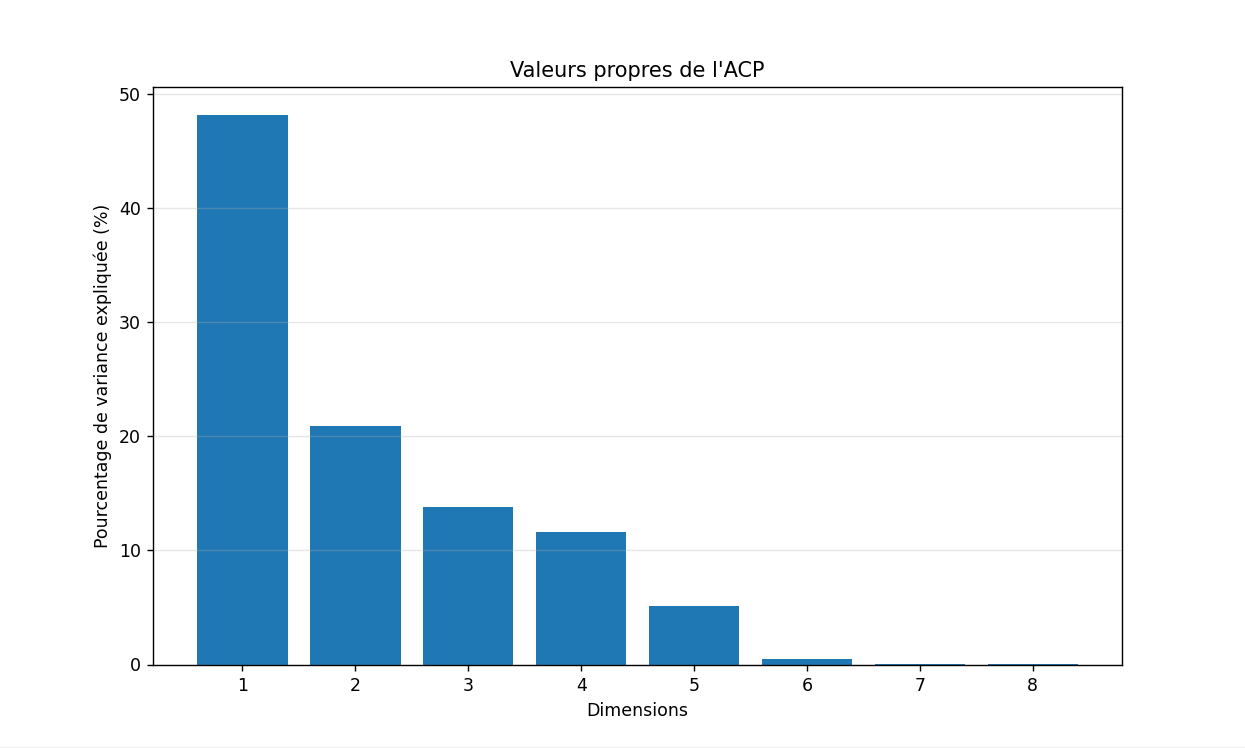
\includegraphics[width=0.75\textwidth]{images/valeurs_propres_ACP.png}
                    \captionof{figure}{}
                \end{center}

            \subsubsection{Interprétation}

        
    \subsection{Analyse catégorielle / qualitative des données}



    %%%%%%%%%%%%%%%%%%%%%%%%%%%%%%%%%%%%%%%%%%%%%%%%%%%%%%%%%%%%%%%%%%%%%%%%%%%%%%%%%%%
    %%%%%%%%%%                            CONCLUSION                         %%%%%%%%%%
    %%%%%%%%%%%%%%%%%%%%%%%%%%%%%%%%%%%%%%%%%%%%%%%%%%%%%%%%%%%%%%%%%%%%%%%%%%%%%%%%%%%

    \section{Conclusion}


\end{document}